%Esto es un comentario :D 
%------------------Encabezado: tiene los paquetes----------------------------------
%Empezamos definiendo que tipo de documento vamos a usar.
%respetar la gerarquía entre corchetes y llaves. Paquetes y especifidad.

\documentclass[onecolumn]{article} %report, book %números de columnos
\usepackage[spanish]{babel} %Para las cosas en español (referencias, etc) Babel puede tener problemas.
%Renombrar los comandos.
\usepackage{multicol} %Paquete para las columnas% 
\usepackage[latin1,utf8]{inputenc} %idioma, latin1:español, inputenc es el paquete de idiomas de occidente %utf8, guión, comas, mayor que, etc, lo que se puede teclar.
\usepackage{graphics,graphicx,xcolor} %xcolor, para colores %figuras
\usepackage{amssymb,amsmath} %Lenguaje matemático %amsmath, el de las integrales
\usepackage{verbatim} %Escribir código
\usepackage{bm} %negrita
\usepackage[a4paper,top=3cm,bottom=3cm,left=2.5cm,right=2.5cm,marginparwidth=1.75cm]{geometry}
%Cambiar margenes, usar más paquetes.
%Fecha en español. Nota: \renewcommand. También paquete para email.
%C y C++, Funciona de manera similar, con paquetes, primero los introducimos.
%Como escribir el simbolo porcentaje sin añadir comentario
%Reducir tamaño de margenes
%Cambiar fuente de letra, tamaño de letra, centrar, alinear a la izquierda, cambiar el temmplate. "centrar section latex"
%Como poner las comillas en español
%Cambiar simbolo de la viñeta

%---------------------------------------------------------------------
\title{Lo que he aprendido sobre Gnuplot}
\author{CARLOS ANDRES RODALLEGA MILLAN}

%---------------------------------------------------------------------
%Toda pareja que comienza con \Begin y termina con \END se llama ENTORNO
%++++++++++++++++++++++CUERPO DEL DOCUMENTO+++++++++++++++++++++++++++
\begin{document}
\maketitle %HAGA el título.... (que está arriba)
%.-.-.-.-.
Este documento resumirá todos los conceptos aprendidos en clase sobre el programa de Gnuplot, como se puede apreciar estará dividido en cada sección con las clases en las cuales se aprendió lo que se esta escribiendo.

\section{Clase 2-16Nov}
El código que se escribió en Atom y se puso en el programa fue el siguiente:
\begin{verbatim}
		#Esto es un comentario en GNUPlot
#Tenemos que decirle que tipo de grafica vamos a realizar (png,jpg, etc), set significa use
set terminal pngcairo #El tipo de gráfico
set output "grafica_16Nov.png" #Nobmre de la gráfica.
#Instrucciones de la gráfica
set xlabel "Eje horizontal"
set ylabel "Eje vertical"
#para pintar se usa el comando plot
plot cos(x)
unset output   #Cerrar archivo
	\end{verbatim}
El resultado de este código fue el siguiente:
\begin{figure}[h!]%[h! here, para la gráfica]
	\centering %para centrar
	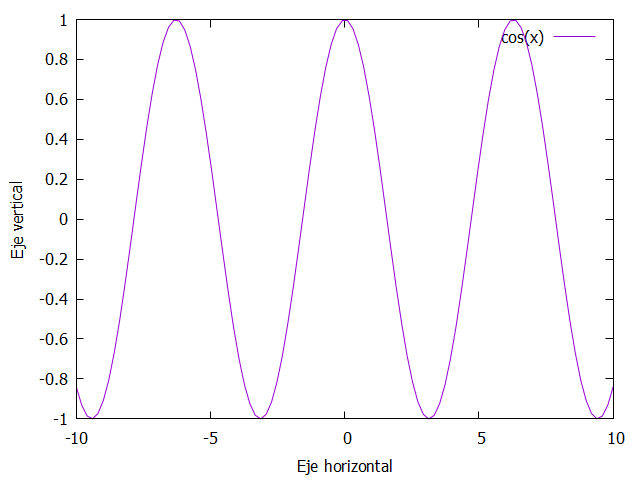
\includegraphics[scale=0.2]{grafica_16Nov.png}
	\caption{\label{fig_cos}Es un archivo .png que contiene la imagen de la función coseno} 
\end{figure}
\subsection{Explicando paso a paso el código anterior}
Lo primero debemos entender que para hacer \textbf{comentarios} usamos \verb+#+ , esta herramienta nos ayuda muchísimo para guiarnos en nuestro código.\\
Debemos especificarle al programa el tipo de gráfica que vamos a realizar, por eso usamos el siguiente comando, en este comando le decimos a Gnuplot que nos cree un archivo .png con el nombre "\textbf{grafica16Nov}":
	\begin{verbatim}
	set terminal pngcairo
	set output "grafica_16Nov.png"
	\end{verbatim}
Ahora le debemos dar las instrucciones de los ejes a nuestro programa, etiquetando los ejes de la siguiente forma:
	\begin{verbatim}
		set xlabel "Eje horizontal"
		set ylabel "Eje vertical"
	\end{verbatim}
Después, debemos decirle al programa la orden a realizar, es decir, que haga la gráfica.
	\begin{verbatim}
		plot cos(x)
	\end{verbatim}
Por último, siempre debemos cerrar nuestro programa.
	\begin{verbatim}
		unset output
	\end{verbatim}
\section{Clase 3-23Nov}
\subsubsection{Primera gráfica de esta clase}
Tengamos en cuenta que aquí en adelante se ignora los comentarios del texto, estos serán puestos en la explicación de paso a paso del código anterior. Presentamos directamente le archivo que se usó esta clase:
	\begin{verbatim}
set terminal pngcairo font "times,26" enhanced color size 900,600
set output "Grafica26Nov.png"
set xrange[-5:5]
set yrange[0:1.2]
set xlabel "x"
set ylabel "P(X)"
set key top right
P1(x)=exp(-x**2)
P2(x)=exp(-(0.7*x)**2)
plot P1(x) w lp ps 2 pt 7 lc 4 t "P_1(X)", P2(x) w l lw 4 t "P_2(X)"
unset output

	\end{verbatim}
El resultado del anterior código es el siguiente:

\begin{figure}[h!]%[h! here, para la gráfica]
	\centering %para centrar
	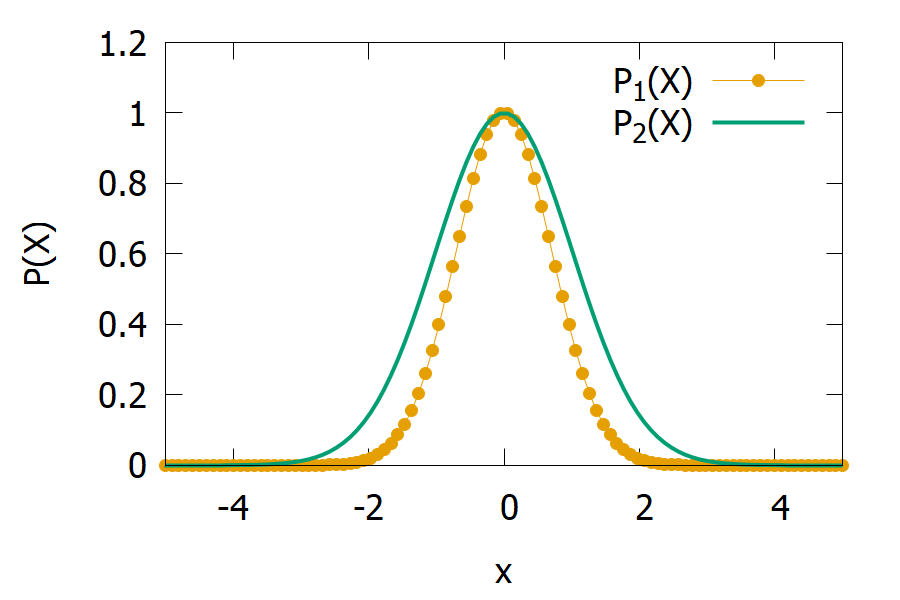
\includegraphics[scale=0.2]{Grafica26Nov.png}
	\caption{\label{fig_exp}Es un archivo .png que contiene la imagen de ambas funciones Gaussianas} 
\end{figure} 
Gnuplot toma x,y,z como los nombres de las variables independientes para cartesianas. (r,t son los nombres de las variables independientes para polares.)
Podemos apreciar que en nuestra anterior gráfica tenemos un estilo y color para cada línea.
\subsection{Ahora vamos a explicar paso a paso el código anterior.}
\begin{verbatim}
set terminal pngcairo font "times,26" enhanced color size 900,600
set output "Grafica26Nov.png"
\end{verbatim}
Como habíamos visto antes, esto nos permite crear y empezar nuestro grafico, con esto, estamos haciendo que lo cree en un archivo .png. Después le estamos especificando el tipo de fuente a usar, el tamaño de fuente y las dimensiones del archivo a realizar.\\
\begin{itemize}
    \item Rango
    \begin{verbatim}
set xrange[-5:5]
set yrange[0:1.2]
set xlabel "x"
set ylabel "P(X)"
	\end{verbatim}
Si no especificamos el rango, este vendrá con valores por defecto de [-10,10] para cada eje coordinado.
    \item Etiquetas de rangos.
\begin{verbatim}
set xrange[-5:5]
set yrange[0:1.2]
set xlabel "x"
set ylabel "P(X)"
\end{verbatim}
Los anteriores comandos, nos permiten asignarle un nombre a cada eje coordinado.
   \item Forma de la línea de nuestra gráfica y graficación.
  \begin{verbatim}
plot P1(x) w lp ps 2 pt 7 lc 4 t "P_1(X)", P2(x) w l lw 4 t "P_2(X)" 
  \end{verbatim}
 En esta línea de códigos le estamos diciendo a Gnuplot que haga las gráficas que están separadas por comas (,) y que las haga de con línea y puntos (\textbf{lp}), después especificamos el tamaño de cada punto (\textbf{"pt7"}), el color "line color" (\textbf{lc 4}) y por último le decimos que le asigne un nombre que se ubica arriba a la derecha \textbf{t "$P(x_1)$"}.\\
lw ancho de la línea.\\
1 morado, 2 verde, 3 azul clarito, 4 naranja.
\end{itemize}
Por último, como hemos venido haciendo, cerramos nuestra gráfica con :
\begin{verbatim}
unset output
\end{verbatim}
\subsection{Segunda gráfica de esta clase "Panal de huevos"}
El archivo usado fue:
\begin{verbatim}
#Grafica en 3d
#Todas las instrucciones que queremos darle a GNUPLOT, las colocaremos siempre en un archivo aparte.
#Eso es un script.
#Enhanced, es para usar subindices o superindices, símbolos.
#Antes de comenzar, colocar/limpiar nuestro espacio. Reset elimina la información en el buffer.
#--------------------Empieza la línea de código----------------
reset

set terminal pngcairo font "Times,26" enhanced color size 900,600

set output "Grafica26_2Nov_3D.png"
set pm3d
set view map
#forma de vista de mapa

#Panal de huevos.
set xlabel "eje x"
set ylabel "eje y"
set xrange[-10:10]
set yrange[-10:10]

f(x,y)=cos(x)*sin(y)
set isosample 500
set ztics 0.5
set cbtics 0.5
#Espacio de las letras de los números del eje z
#Lo anterior organiza la vista.
#isosample es una grilla, cantidad de línea, 50 líneas por variable inde.
unset surface
splot f(x,y) t" "

#Pareja pm3d, para pintarlo, aparecen colores y la escala.
#Unset surface, para quitar la malla
#x al cuadrado
unset output

\end{verbatim}
El grafico realizado fue el siguiente:
\begin{figure}[h!]
	\centering
	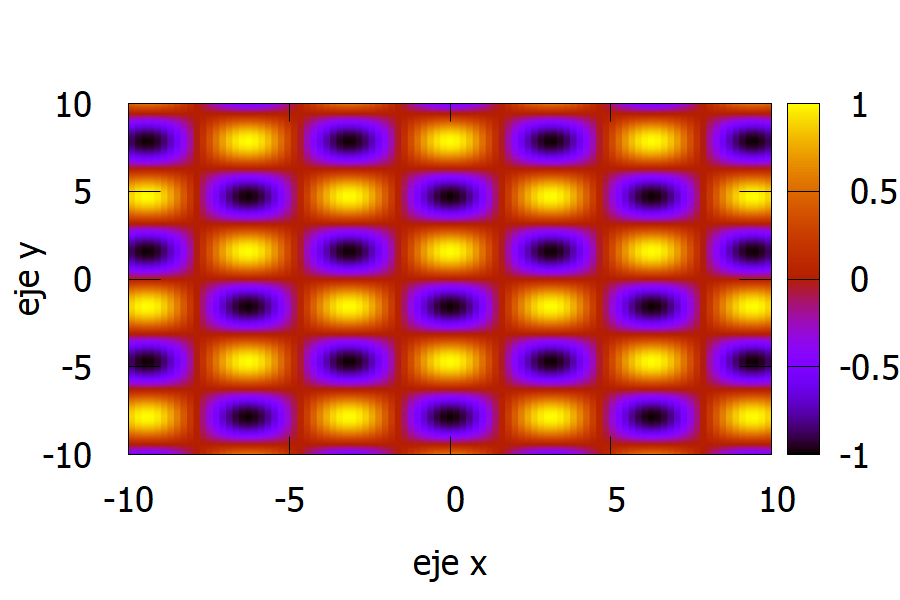
\includegraphics[scale=0.2]{Grafica263D.png}
	\caption{\label{fig_3d}Esta fue la figura realizada en 3d con el anterior código, vista desde arriba.}
\end{figure}

Texto por si acaso 
\subsection{Ahora vamos a explicar paso a paso el código anterior.}

\section{Clase Revelo}
El siguiente archivo es interesante porque se puede crear diferentes gráficas en  una misma gráfica.
Presentamos directamente le archivo que Revelo nos pasó para esta clase:
	\begin{verbatim}

set terminal pngcairo transparent enhanced font "Times-New-Roman,12" 
set output "grafica1_clase4.png"

set xrange[0:2*pi]
set yrange[-1.1:1.1]
set xlabel "Angulo ({/Symbol Q})"
set ylabel "Eje vertical"
set key bottom left
plot sin(x)

unset output 
reset

#grafica 3d
set terminal pngcairo transparent enhanced font "Times-New-Roman,14"
set output "grafica3D_clase4.png"
\end{verbatim}
\begin{multicols}{3}
\begin{verbatim}
set multiplot 

set origin 0,0
set size 0.5,0.5
set pm3d map
set hidden3d
set isosamples 150
set xrange[0:2*pi]
set yrange[-2*pi:2*pi]
set zrange[-1:1]
set cbrange[-1:1]
splot sin(x)*cos(y)

reset

set origin 0.5,0
set size 0.5,0.5
set hidden3d
set isosamples 150
set xrange[-0.5*pi:0.5*pi]
set yrange[0:4*pi]
splot sin(x)*cos(y)

reset

set origin 0,0.5
set size 0.5,0.5
set pm3d
unset surface
set isosamples 150
set xrange[0:2*pi]
set yrange[-2*pi:2*pi]
set ztics 0.5
set cbtics 0.5
unset key
splot sin(x)*cos(y)

reset

set origin 0.5,0.5
set size 0.5,0.5
set pm3d at bs
unset surface
set isosamples 150
set xrange[0:2*pi]
set yrange[-2*pi:2*pi]
set ztics 0.5
set cbtics 0.5
unset key
splot sin(x)*cos(y)

unset multiplot

unser output 
	\end{verbatim}
\end{multicols}{2}
\subsection{Ahora vamos a explicar paso a paso el código anterior.}

para windows: powershell
en la powershell wgnuplot Clase4gnuplot.plt
\section{Libro que dejó la profesora}

\end{document}
